\chapter{Introduction to Linear Algebra}

Welcome to the world of linear algebra, a branch of mathematics that relies on vectors, matrices, and linear transformations. You are familiar with most of these concepts, so in this workbook you’ll see how you can use them together to solve problems.  

Let’s review what you know.

\begin{itemize}
\item \textbf{Vectors}. In workbook 5, you saw how vectors can represent forces and then how to add and multiply them to figure out such things as rocket engine force and direction. 
\item \textbf{Matrices}. In workbook 8 you learned to use spreadsheets to solve problems numerically, like how to figure out the number of barrels a cooper has to produce to achieve a certain take-home pay. Spreadsheets are essentially matrices—a row by column structure that contains values. 
\item \textbf{Linear transformations}. When you studied congruence in workbook 4, you were introduced to a few linear transformations such as translation and reflection. 
\end{itemize}

\section{What's With the Linear?}

You might be thinking, “Hey, haven’t I’ve been doing algebra already?” 

You have. You've come a long way in your problem solving journey. You've used algebra to solve simple equations like $7x + 10 = 24$ and quadratic equations like $4x^{2} + 9x + 31 = 0$. What distinguishes linear algebra is that linear combinations are at its heart. Any equation with a power greater than 1, like a quadratic, is nonlinear.

We’ll first take a look at linear combinations

\section{Linear Combinations}

You won’t see any \textbf{sin}, \textbf{cos}, or \textbf{tan} operations in this section. Linear operations do NOT use trigonometric functions. Those are all nonlinear. A linear combination  preserves addition and scalar multiplication. You will see that linear combinations allow you to solve many types of problems in science and engineering. Before we get deep into the numbers, let’s take a look at a few linear operations you can perform on images. This will give you an intuition for the underlying math. Then we’ll take a look at some numbers.

\section{Image Operations}
The simplest image, a bitmap, can be represented by a two-dimensional matrix of values, either 0, for black, or 1, for white. Grayscale images are also represented by a two-dimensional matrix of values, but the values typically range from 0 to 255. Zero is black, 255 is white, the values in between represent shades of gray. 

Color images are more complex. The simplest color image is a three-dimensional matrix of values. You can think of it as three 2D matrices, one to represent red values (R), another for green values (G), and the third for blue values (B). The combination of R, G, and B determines the color you see.

Working with images, means working with millions of pixels. Fortunately modern techniques make this a snap. Let's look at some common operations on an image of a rocket.

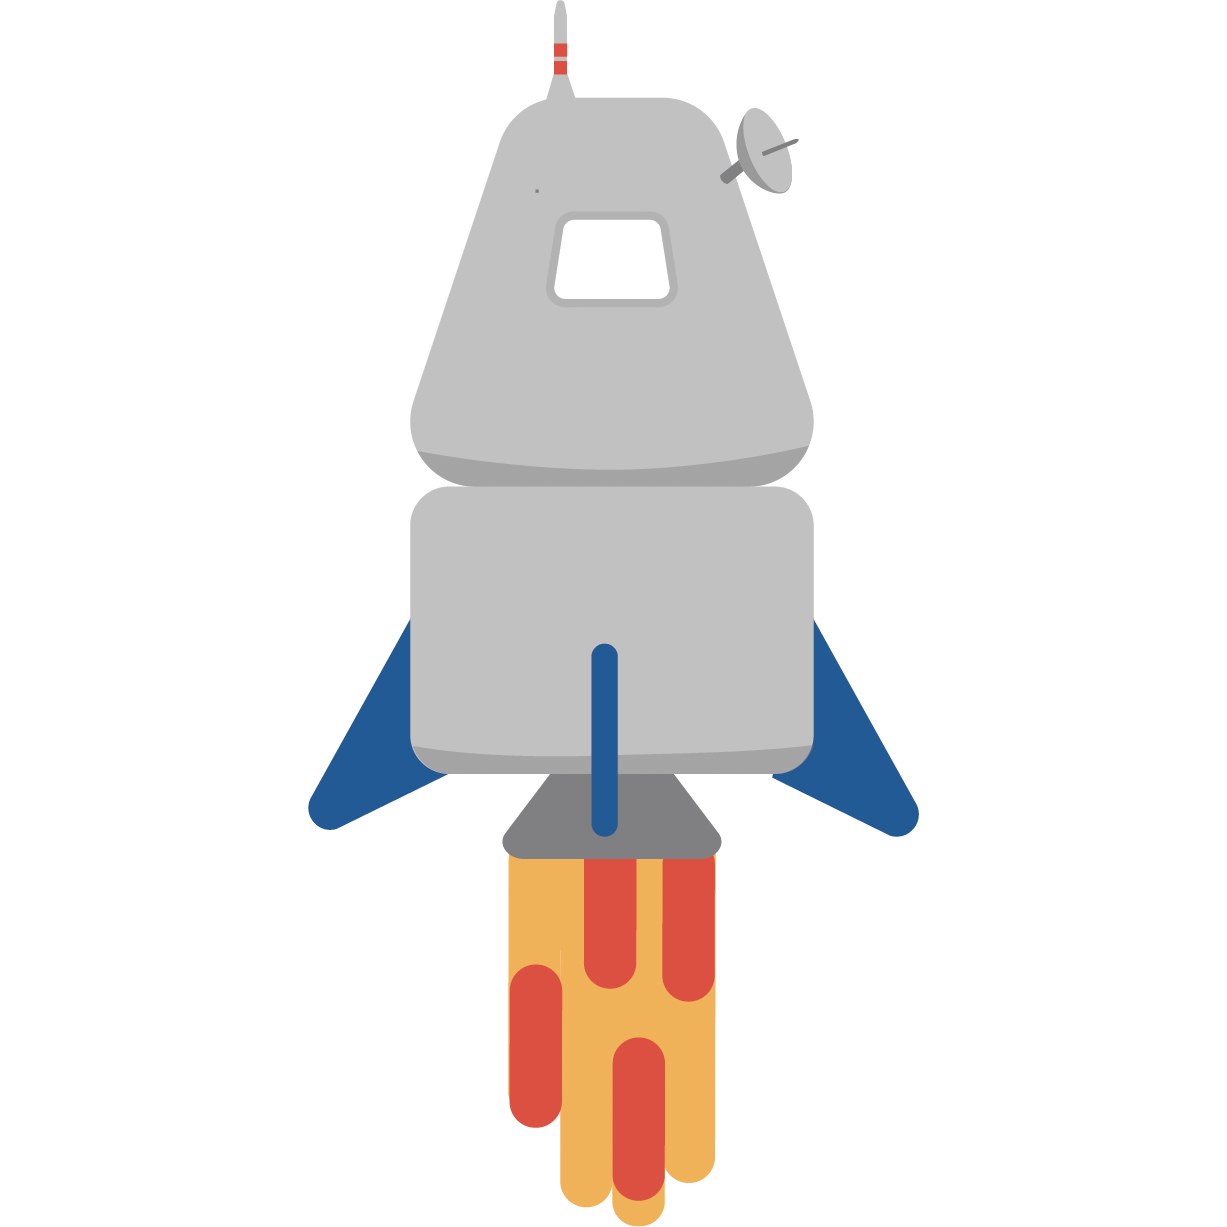
\includegraphics[width=0.25\textwidth]{flying-rocket.png}

Flipping is a linear operation.

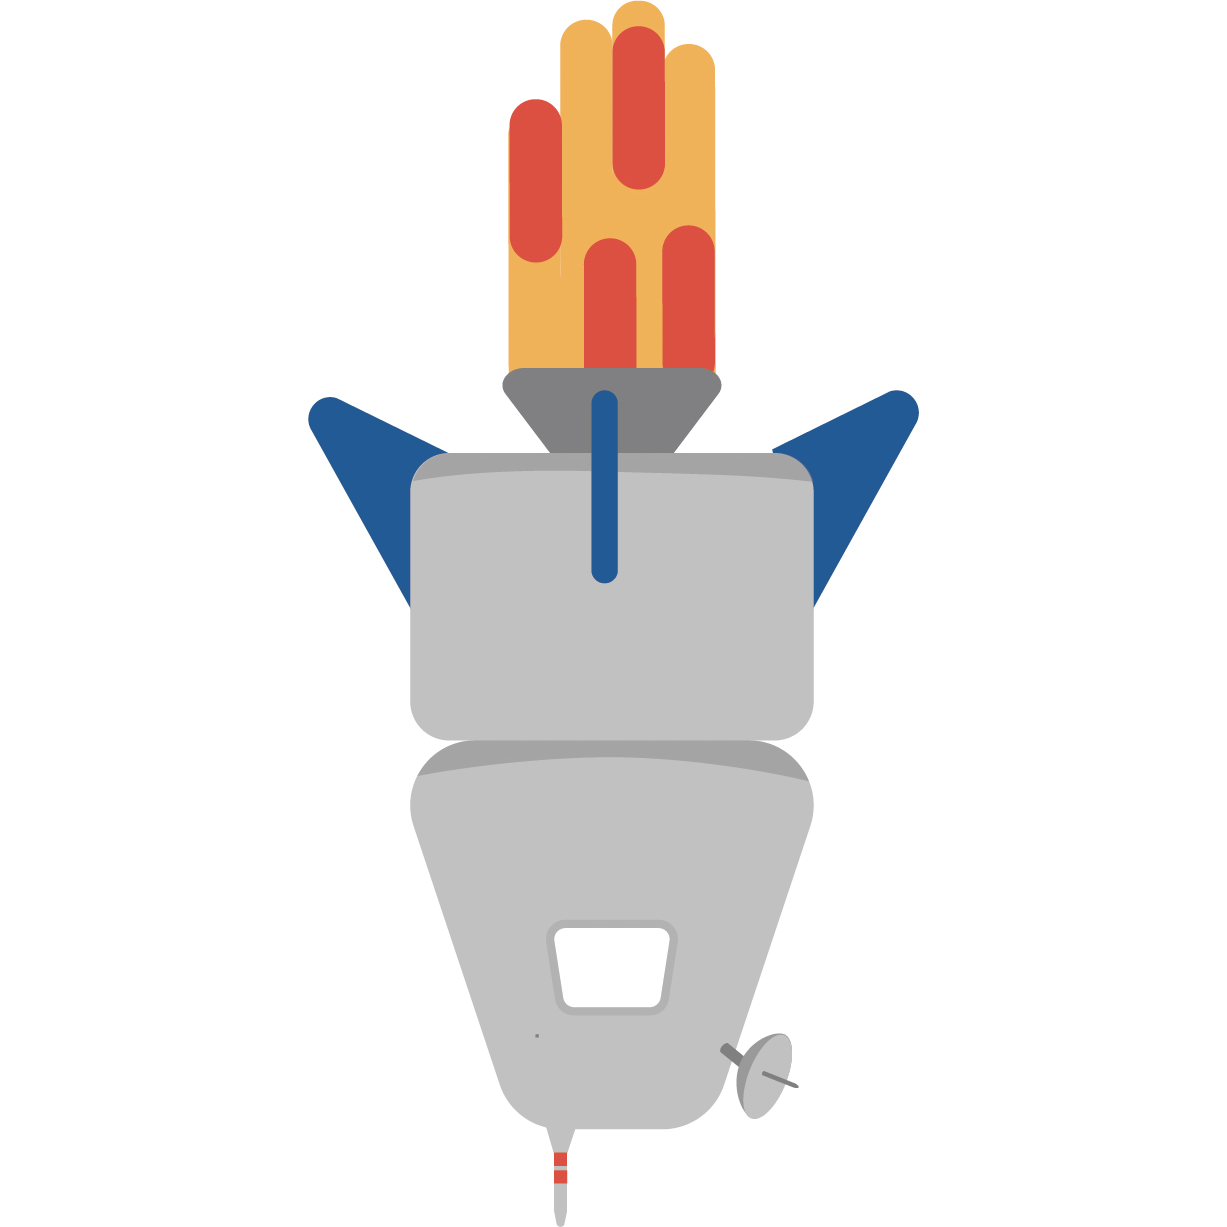
\includegraphics[width=0.25\textwidth]{rocket-flipped.png}

Next, the image is rotated 90 degrees. This rotation is linear, but if you want to rotate it at an angle that isn't a multiple of 90, you would need trigonometry. You'd be treading into nonlinear territory. But that happens in the field of linear algebra. You'll learn about nonlinear extensions later that use trigonometric functions and imaginary numbers.

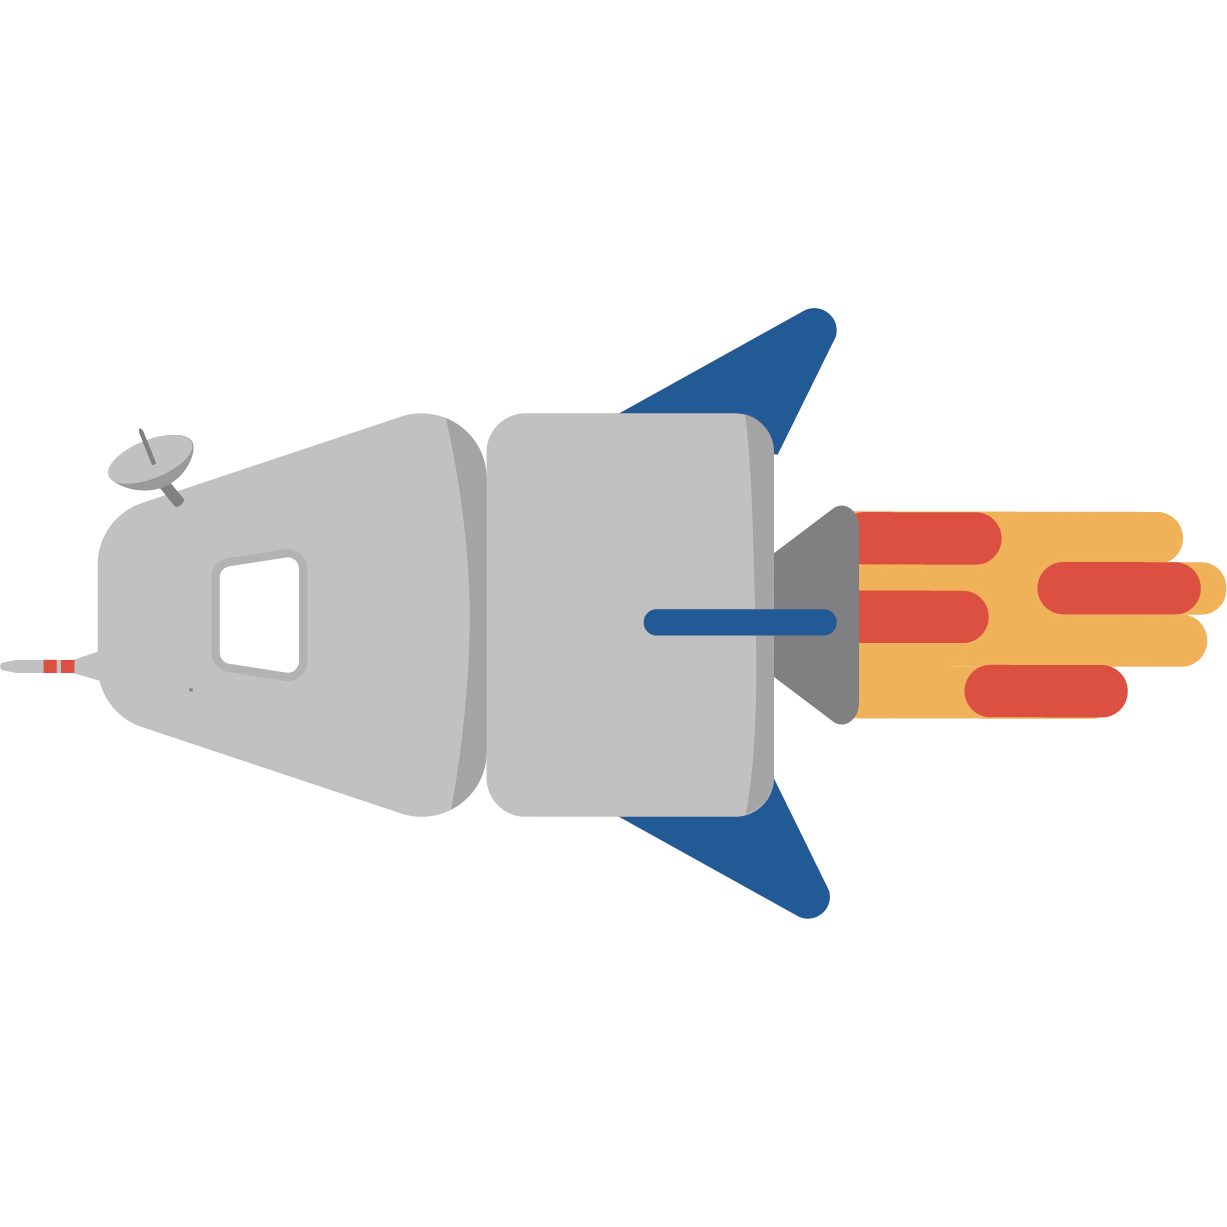
\includegraphics[width=0.25\textwidth]{rocket-rotated-90.png}

Inversion is an interesting linear operation that involves redefining the red, green and blue values such that the new value is 1.0 minus the old value. The resulting black background gives the impression the rocket is in deep space, don't you think?

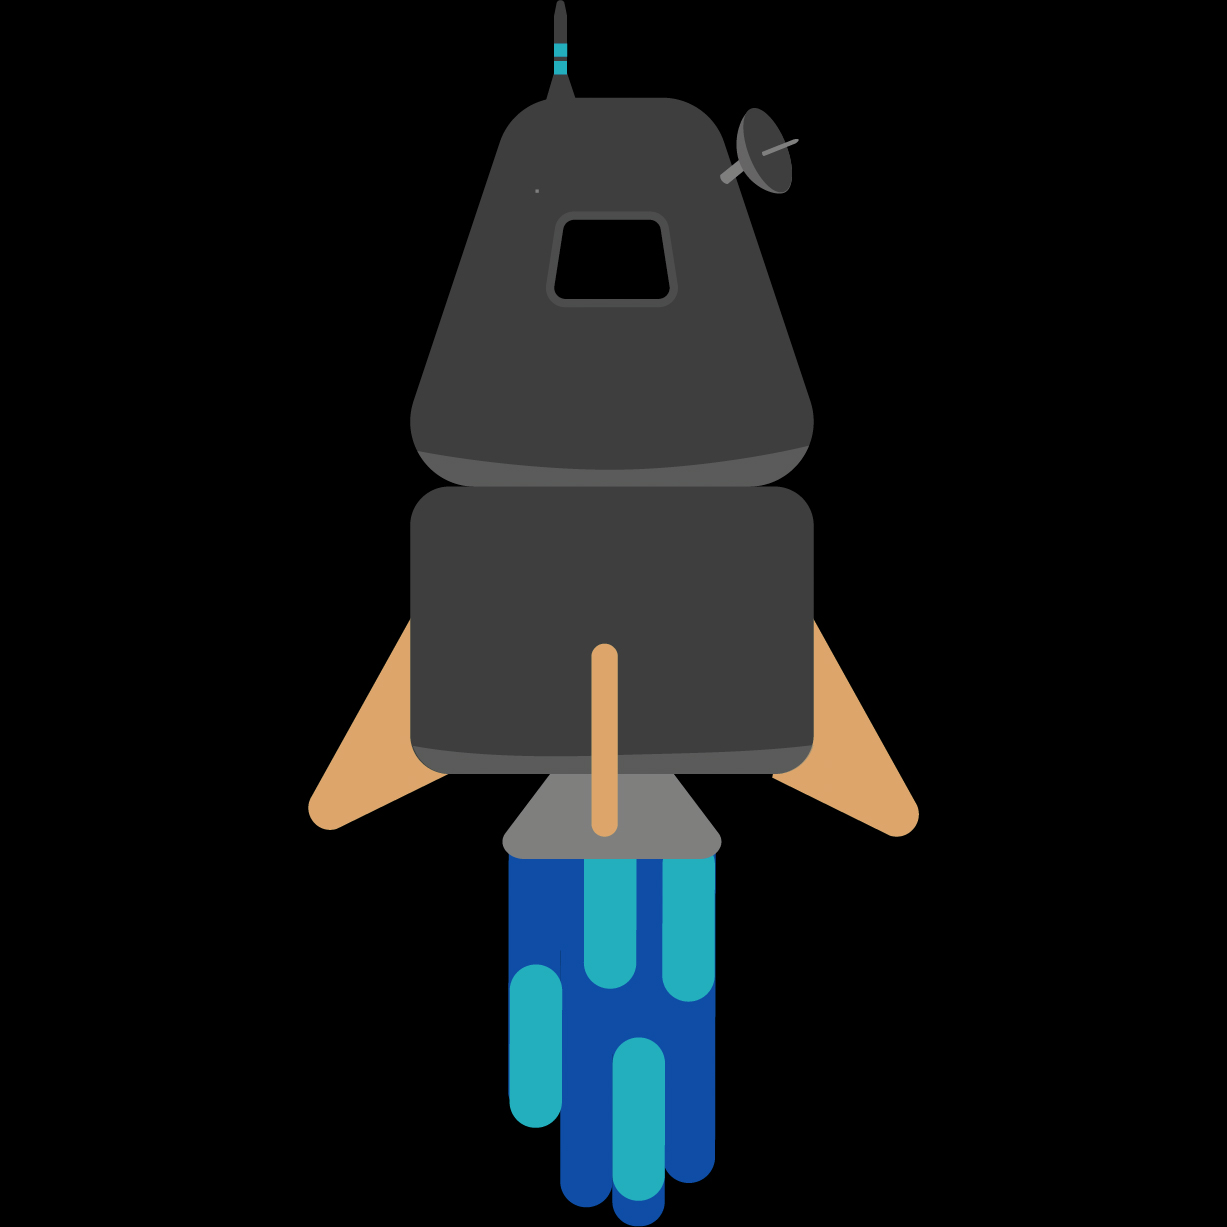
\includegraphics[width=0.25\textwidth]{rocket-inverted.png}

It is possible to redefine the red, green, and blue values in many ways. Visit the NASA website and search for false color images. NASA and other scientists redefine colors to communicate such things as the amount of vegetation or water in an area, the temperatures of the sun's surface, and so on. Photographers often do this for artistic effect. For example, the image on the left was taken with an infrared camera. (But not the thermal infrared you've seen. This is the infrared that's emitted by living plants.) The image is further processed to swap channels. For example, the matrix representing red might be swapped with the matrix representing blue. The image on the right shows the image after swapping color values. All these swapping operations are linear.

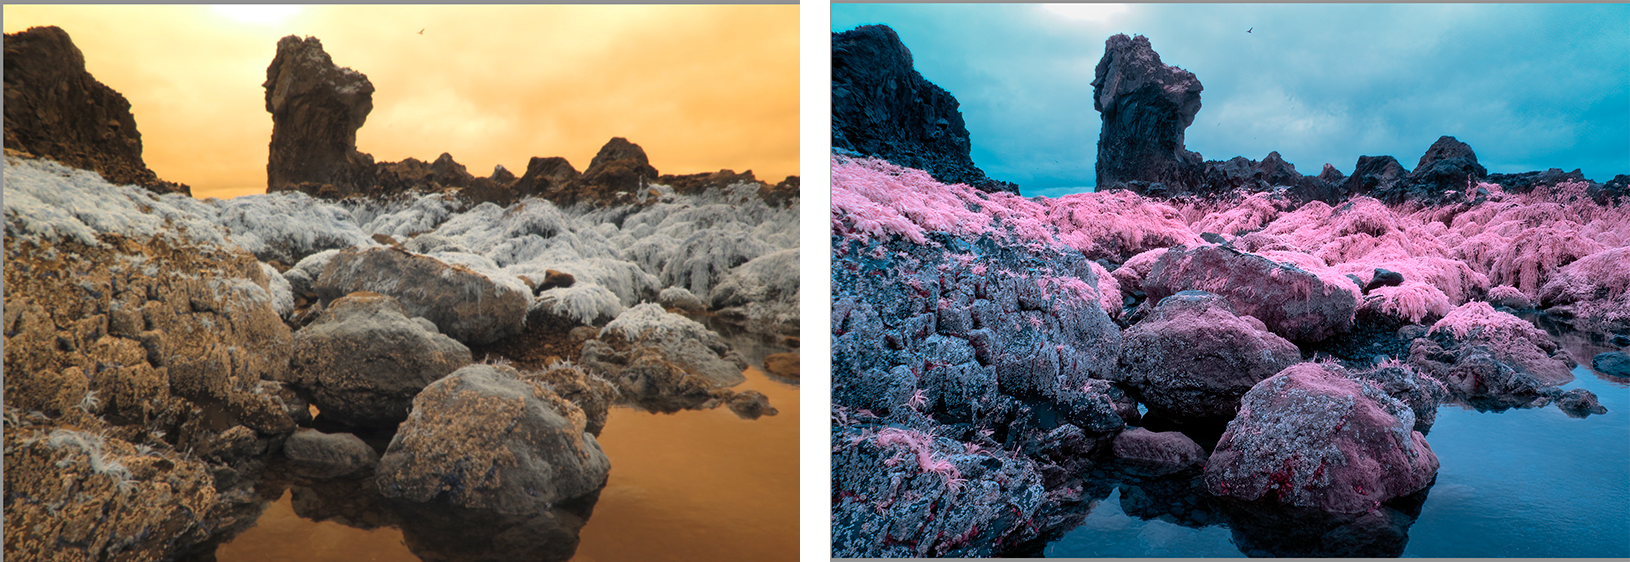
\includegraphics[width=1.0\textwidth]{infrared.png}

\section{The Numbers Behind Some Image Operations}

You'll see a few matrices in this section. Let's first see how a spreadsheet can be represented as a matrix. Recall the barrel making shop example. This is part of that spreadsheet. 

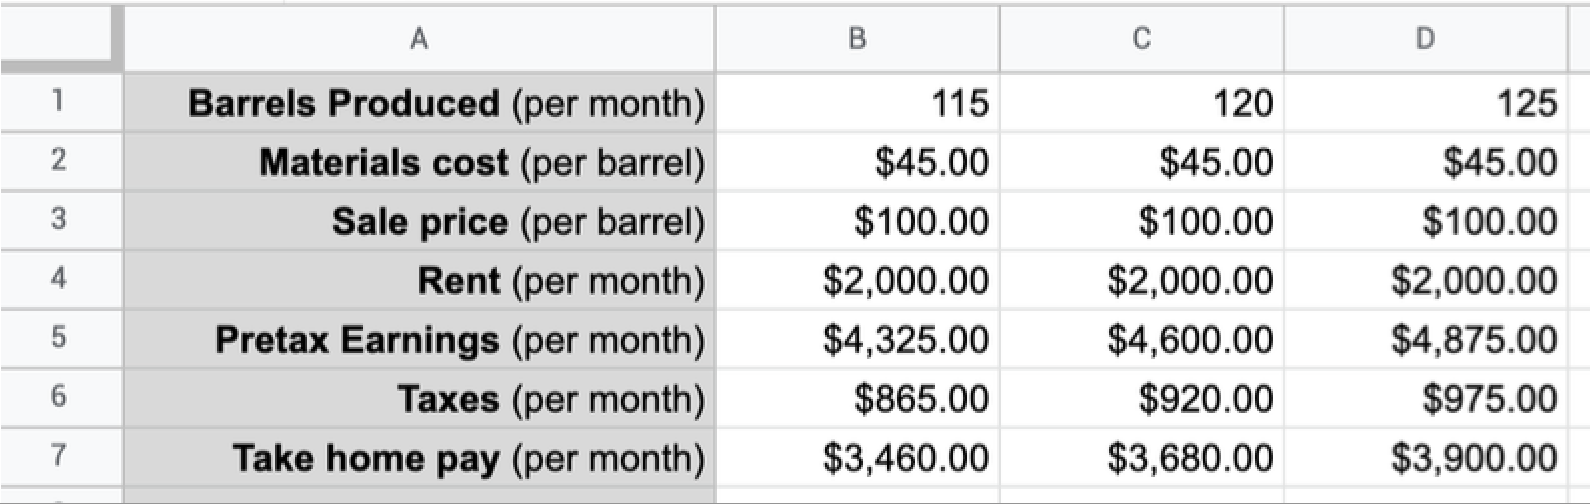
\includegraphics[width=1.0\textwidth]{spreadsheet.png}

Represented as a matrix, it looks like the following. Note the differences. A matrix contains only values, no labels. This matrix uses floating point values, hence the inclusion of decimal points. 

$$\begin{bmatrix}
115. & 120. & 125.\\
45.0 & 45.0 & 45.0\\
100.0 & 100.0 & 100.0\\
2000. & 2000. & 2000.\\
4325. & 4600. & 4875.\\
865. & 920. & 975.\\
3460. & 3680. & 3900.
\end{bmatrix}$$
 
A matrix that represents an image contains only pixel values, whereas the barrel making shop matrix represents seven kinds of variables: barrels produced, materials cost, sales price, rent, pretax earnings, taxes, and take home pay. 

The simplest image to create is a bitmap because that requires a matrix of zeros and ones. This is a matrix for a 10 pixel by 10 pixel image. Why the decimal points when this is obviously a matrix of integers? It turns out that when you use tools like python to process matrices, you must be conscious of data types. I already know that most of the python methods I use for image operations expect floating points. A few expect integer types, but you'll see how to handle type conversion later, in the section on python. 

$$\begin{bmatrix}
0. & 0. & 0. & 0. & 1. & 0. & 0. & 0. & 1. & 0\\
0. & 0. & 0. & 0. & 1. & 1. & 1. & 1. & 1. & 1\\
0. & 0. & 0. & 0. & 1. & 0. & 0. & 0. & 1. & 0\\
0. & 0. & 0. & 0. & 1. & 0. & 0. & 0. & 1. & 0\\
0. & 0. & 0. & 0. & 1. & 0. & 0. & 0. & 1. & 0\\
0. & 0. & 0. & 0. & 1. & 0. & 0. & 0. & 1. & 0\\
0. & 0. & 0. & 0. & 1. & 0. & 0. & 0. & 1. & 0\\
0. & 0. & 0. & 0. & 1. & 1. & 1. & 1. & 1. & 1\\
0. & 0. & 0. & 0. & 1. & 0. & 0. & 0. & 1. & 0\\
0. & 0. & 0. & 0. & 1. & 0. & 0. & 0. & 1. & 0
\end{bmatrix}$$

When converted to an image, it is very tiny. This is an enlarged version so you can see the pattern.


\includegraphics[width=0.25\textwidth]{normal.png}

We can create an inverse of this image by changing all the values in the matrix so that 0 becomes 1 and 1 becomes 0. (Technically this is not the way you'd invert a matrix, as you'll see in the python section. For this example, you will get the same visual result, but when you start inverting matrices programmatically, you will learn the formal definition.)

$$\begin{bmatrix}
1. & 1. & 1. & 1. & 0. & 1. & 1. & 1. & 0. & 1\\
1. & 1. & 1. & 1. & 0. & 0. & 0. & 0. & 0. & 0\\
1. & 1. & 1. & 1. & 0. & 1. & 1. & 1. & 0. & 1\\
1. & 1. & 1. & 1. & 0. & 1. & 1. & 1. & 0. & 1\\
1. & 1. & 1. & 1. & 0. & 1. & 1. & 1. & 0. & 1\\
1. & 1. & 1. & 1. & 0. & 1. & 1. & 1. & 0. & 1\\
1. & 1. & 1. & 1. & 0. & 1. & 1. & 1. & 0. & 1\\
1. & 1. & 1. & 1. & 0. & 0. & 0. & 0. & 0. & 0\\
1. & 1. & 1. & 1. & 0. & 1. & 1. & 1. & 0. & 1\\
1. & 1. & 1. & 1. & 0. & 1. & 1. & 1. & 0. & 1
\end{bmatrix}$$

When converted to an image and enlarged, it looks like this:


\includegraphics[width=0.25\textwidth]{inverse.png}

Rotating the original matrix by 90 degrees gives this:

$$\begin{bmatrix}
0. & 1. & 0. & 0. & 0. & 0. & 0. & 1. & 0. & 0.\\
1. & 1. & 1. & 1. & 1. & 1. & 1. & 1. & 1. & 1.\\
0. & 1. & 0. & 0. & 0. & 0. & 0. & 1. & 0. & 0.\\
0. & 1. & 0. & 0. & 0. & 0. & 0. & 1. & 0. & 0.\\
0. & 1. & 0. & 0. & 0. & 0. & 0. & 1. & 0. & 0.\\
1. & 1. & 1. & 1. & 1. & 1. & 1. & 1. & 1. & 1.\\
0. & 0. & 0. & 0. & 0. & 0. & 0. & 0. & 0. & 0.\\
0. & 0. & 0. & 0. & 0. & 0. & 0. & 0. & 0. & 0.\\
0. & 0. & 0. & 0. & 0. & 0. & 0. & 0. & 0. & 0.\\
0. & 0. & 0. & 0. & 0. & 0. & 0. & 0. & 0. & 0.
\end{bmatrix}$$

This is the resulting enlarged image:


\includegraphics[width=0.25\textwidth]{rotate90.png}

You'll transpose many matrices in the upcoming pages. It requires swapping rows for columns. 

$$\begin{bmatrix}
0. & 0. & 0. & 0. & 0. & 0. & 0. & 0. & 0. & 0.\\
0. & 0. & 0. & 0. & 0. & 0. & 0. & 0. & 0. & 0.\\
0. & 0. & 0. & 0. & 0. & 0. & 0. & 0. & 0. & 0.\\
0. & 0. & 0. & 0. & 0. & 0. & 0. & 0. & 0. & 0.\\
1. & 1. & 1. & 1. & 1. & 1. & 1. & 1. & 1. & 1.\\
0. & 1. & 0. & 0. & 0. & 0. & 0. & 1. & 0. & 0.\\
0. & 1. & 0. & 0. & 0. & 0. & 0. & 1. & 0. & 0.\\
0. & 1. & 0. & 0. & 0. & 0. & 0. & 1. & 0. & 0.\\
1. & 1. & 1. & 1. & 1. & 1. & 1. & 1. & 1. & 1.\\
0. & 1. & 0. & 0. & 0. & 0. & 0. & 1. & 0. & 0.
\end{bmatrix}$$

The resulting image looks like this:


\includegraphics[width=0.25\textwidth]{transpose.png}

What about adding images? That fits the definition of a linear combination. Recall that grayscale images have values from 0 to 255. To make things simple, let's define two matrices with values ranging from 0.0 to 1.0. When we want a grayscale image, it's easy to multiply the matrix by 255. 

Let's call this matrix f.

$$\begin{bmatrix}
1.0 & 0.5 & 0.0\\
1.0 & 1.0 & 1.0\\
0.5 & 0.0 & 0.0 
\end{bmatrix}$$

When multiplied by 255 and converted to a grayscale image:


\includegraphics[width=0.25\textwidth]{fBitmap.png}

Let's call this matrix g:

$$\begin{bmatrix}
0.5 & 0.0 & 0.0\\
1.0 & 0.5 & 1.0\\
1.0 & 1.0 & 1.0 
\end{bmatrix}$$

When multiplied by 255 and converted to a grayscale image:


\includegraphics[width=0.25\textwidth]{gBitmap.png}

When we add f and g we get k:

$$\begin{bmatrix}
1.5 & 0.5 & 0.0\\
2.0 & 1.5 & 2.0\\
1.5 & 1.0 & 1.0 
\end{bmatrix}$$

But the values in k exceed the range of 0.0 to 1.0, so we normalize by dividing the matrix by 1.0

$$\begin{bmatrix}
0.75 & 0.25 & 0.00\\
1.00 & 0.75 & 1.00\\
0.75 & 0.50 & 0.50  
\end{bmatrix}$$

When multiplied by 255 and converted to grayscale, we get:


\includegraphics[width=0.25\textwidth]{fgBitmapAdded.png}

Let's go back to the first small grayscale image:


\includegraphics[width=0.25\textwidth]{fBitmap.png}

If you want to keep the pattern in the first column, you could multiply the matrix by a vector, [1.0, 0.0, 0.0]. The 1.0 will keep the values in the first column, but the 0.0 will knock out the other values because 0.0 times anything equals 0.0.


\includegraphics[width=0.25\textwidth]{onechannel.png}

What do you think will happen if you use the vector [0.0, 1.0, 0.0] or [0.0, 0.0, 1.0]? You'll get a chance later to use python to perform image operations.

All the operations we performed on these images satisfy the requirement for linear combinations: preserving addition and scalar multiplication. 


\section{Applications of Linear Algebra}

So far you've seen how linear operations on matrices can process images by:
\begin{itemize}
\item multipling a matrix using a scalar (e.g., normalize, change the range)
\item adding one matrix to another to get a composite image 
\item multipling two matrices to perform a transform (e.g., flipping)
\item mulitpliing a matrix with a vector (isolating a channel)
\end{itemize}

Many areas in engineering and science rely on the matrix operations defines by linear algebra. Besides image processing, linear algebra is used for: 
\begin{itemize}
\item Computer Graphics. When you play a video game or watch the latest CG animation, matrix operations transform objects in the scene to make them appear as if moving, getting closer, and so on. You can represent the vertices of objects as vectors, and then apply a transformation matrix.
\item Data Analysis. We live in an era in which it's easy to collect so much data that it's difficult to make sense of the data by just looking at it. You can represent the data in matrix form and then find a solution vector. For example, scientists use this technique to figure out the effectiveness of drug treatments on disease.
\item Economics. Take a look at financial section of any news organization and you'll see headlines such as "Economic Data Points to Faster Growth" or "Is the Inflation Battle Won?" Economists can use systems of linear equations to represent economic indicators, such as consumer consumption, government spending, investment rate, and gross national product. By using various methods that you'll learn about later, they can get a good idea of the state of the economy.
\item Engineering. Engineers couldn't do without linear algebra. For example, the orbital dynamics of space travel relies on it. Engineers must predict and calculate the the motion of planetary bodies, satellites, and spacecraft. By solving systems of linear equations engineers can make sure that a spacecraft travels to its destination without running into a satellite or space rock.
\end{itemize}

\section{Let's Observe the Sun!}
India recently sent the Aditya spacecraft on a mission to study the Sun. Without a thorough understanding of linear algebra (among other things), the engineers would not have accomplished the amazing feat of getting Aditya in a stable orbit around a Lagrange point. In previous chapters you learned about gravity and its effects. 

A Lagrange point is a point in space between two bodies (e.g. Earth and Sun) where there is gravitational equilibrium. With the right trajectory, a spacecraft will orbit around a Lagrange point in a stable position that doesn’t require much energy to maintain. That’s called a Halo orbit. Because that there are no fueling stations in space, a Halo orbit will allow Aditya to maintain position for about 5 years. Pretty good mileage!

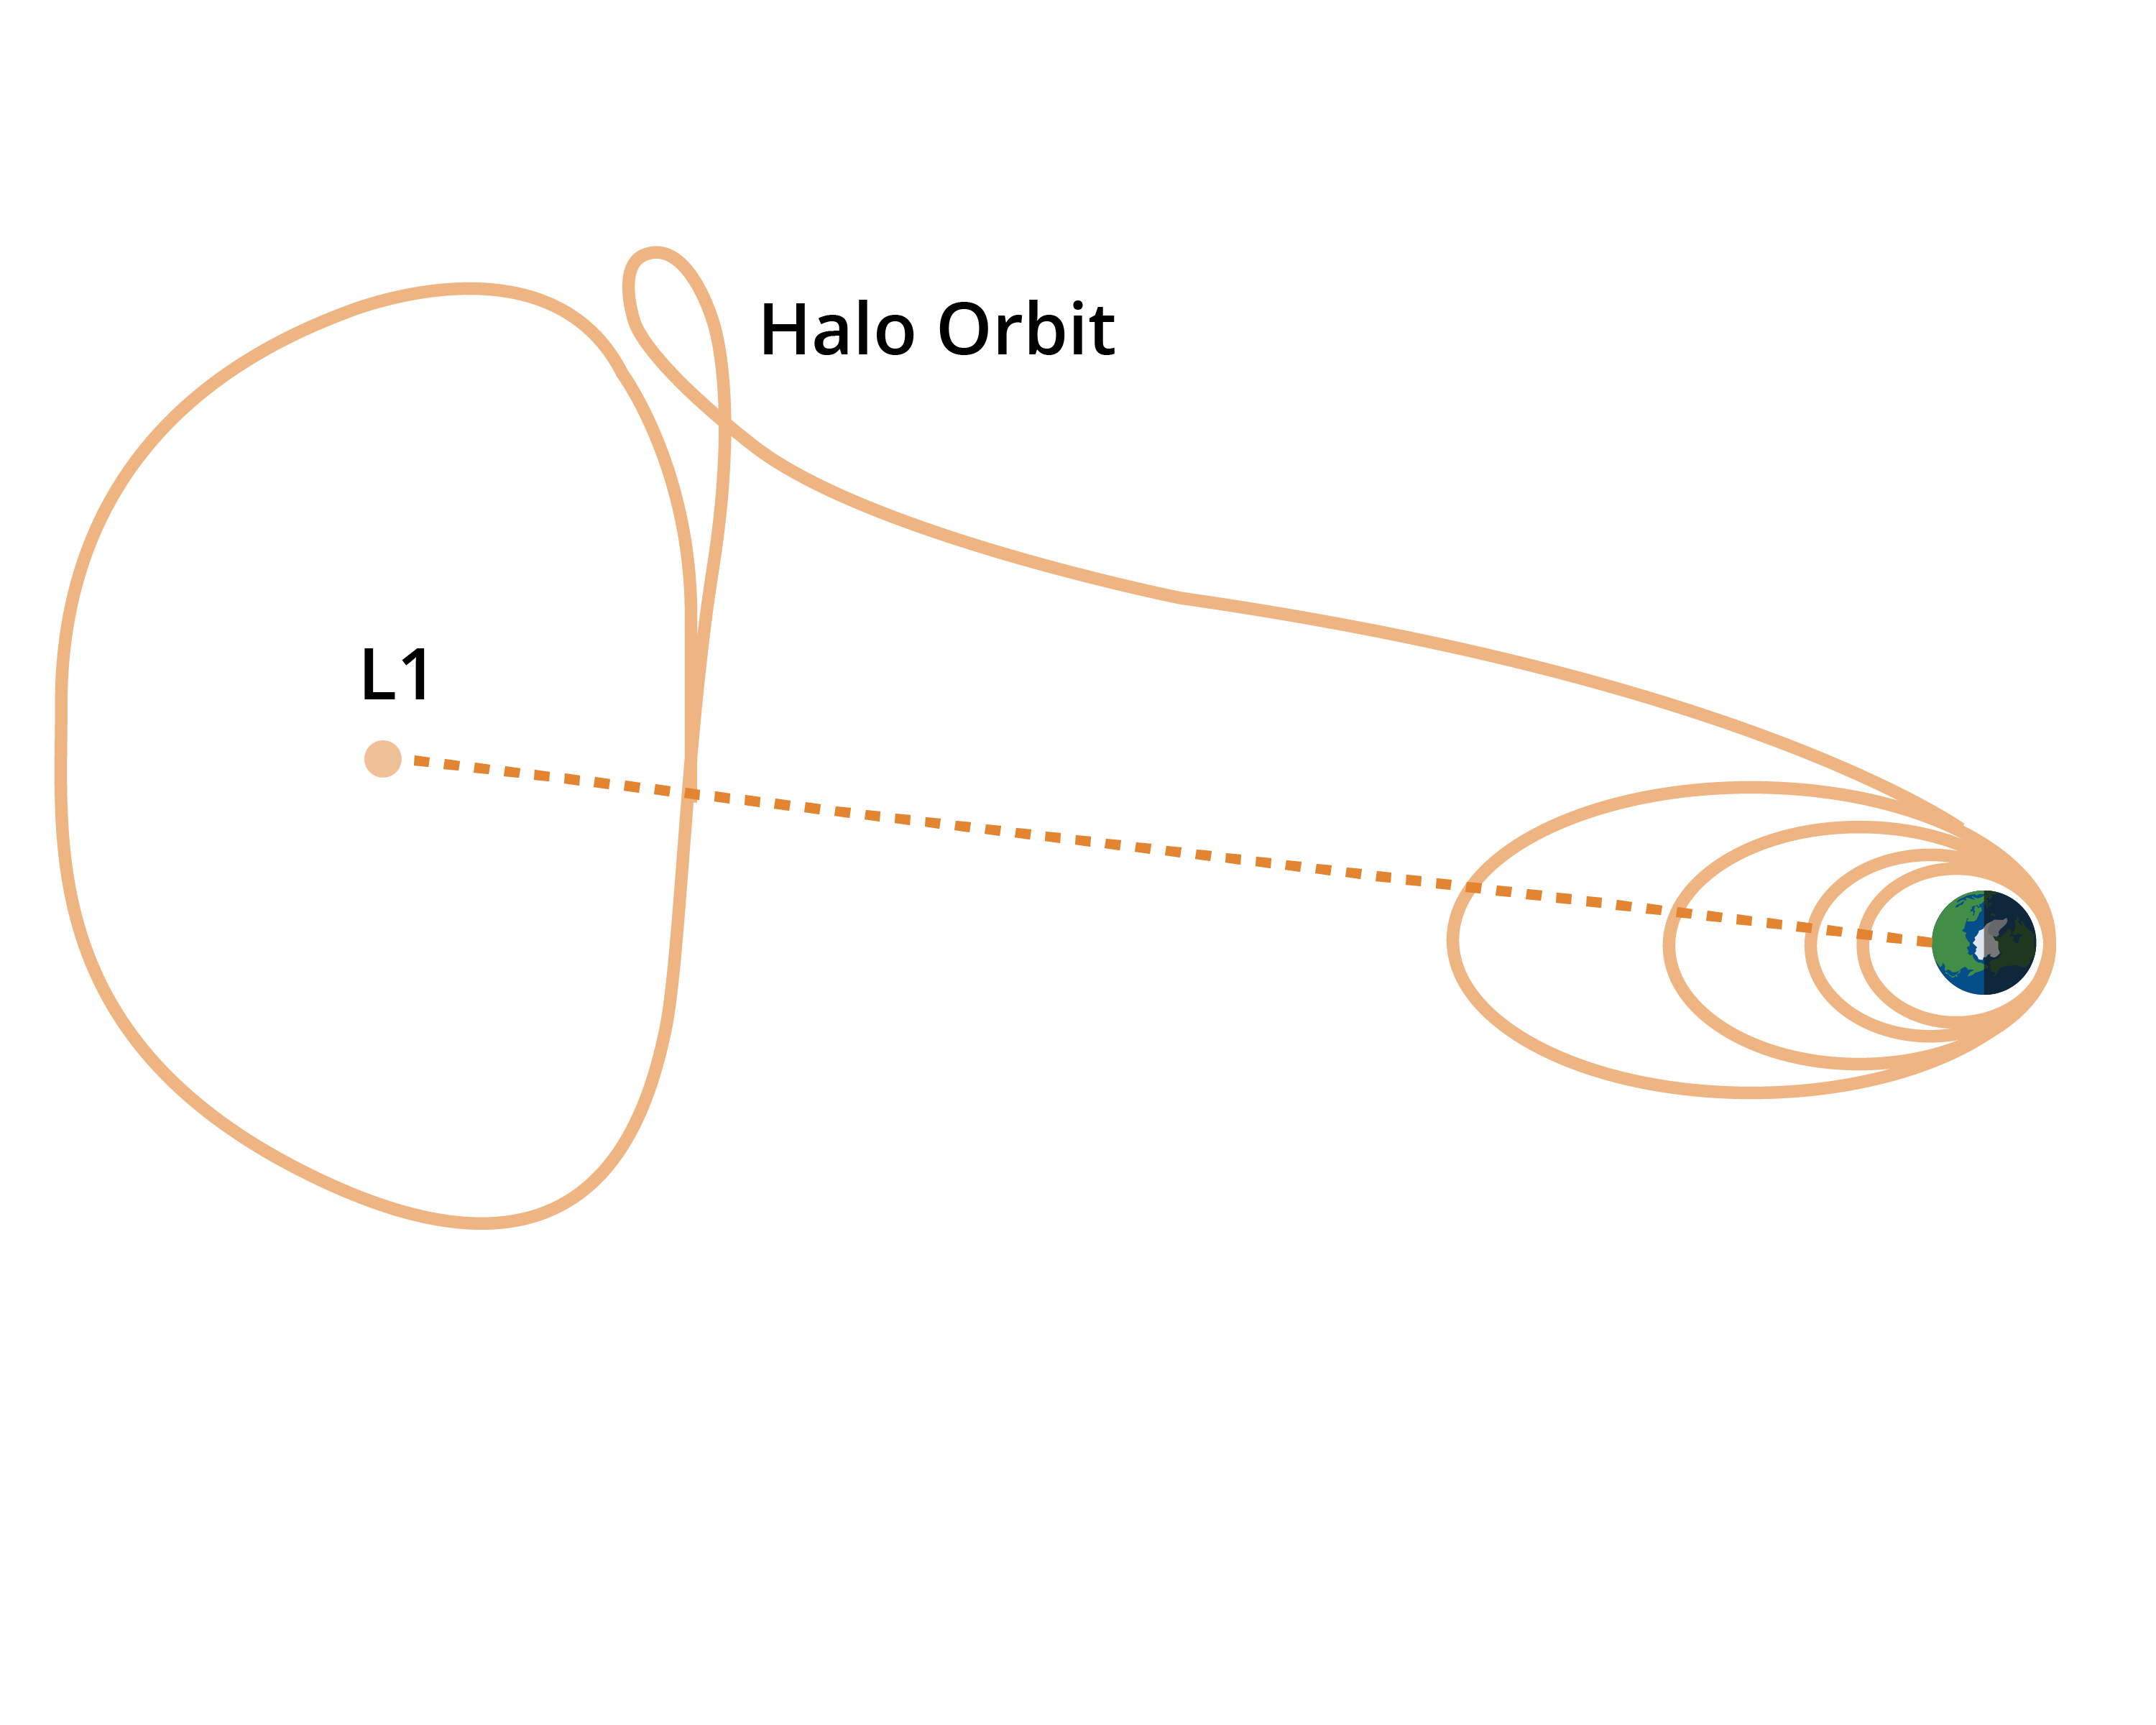
\includegraphics[width=0.5\textwidth]{orbit.png}

Aditya’s engineers had to calculate a looping maneuver that would precisely inject the Aditya spacecraft into the Halo orbit. They determined the angles and burn times for the thrust engine. If they were wrong in one direction, the spacecraft would fly off to the sun. The other direction would send the spacecraft back in the direction of Earth. Their success is due to a solid understanding of vectors and linear algebra.

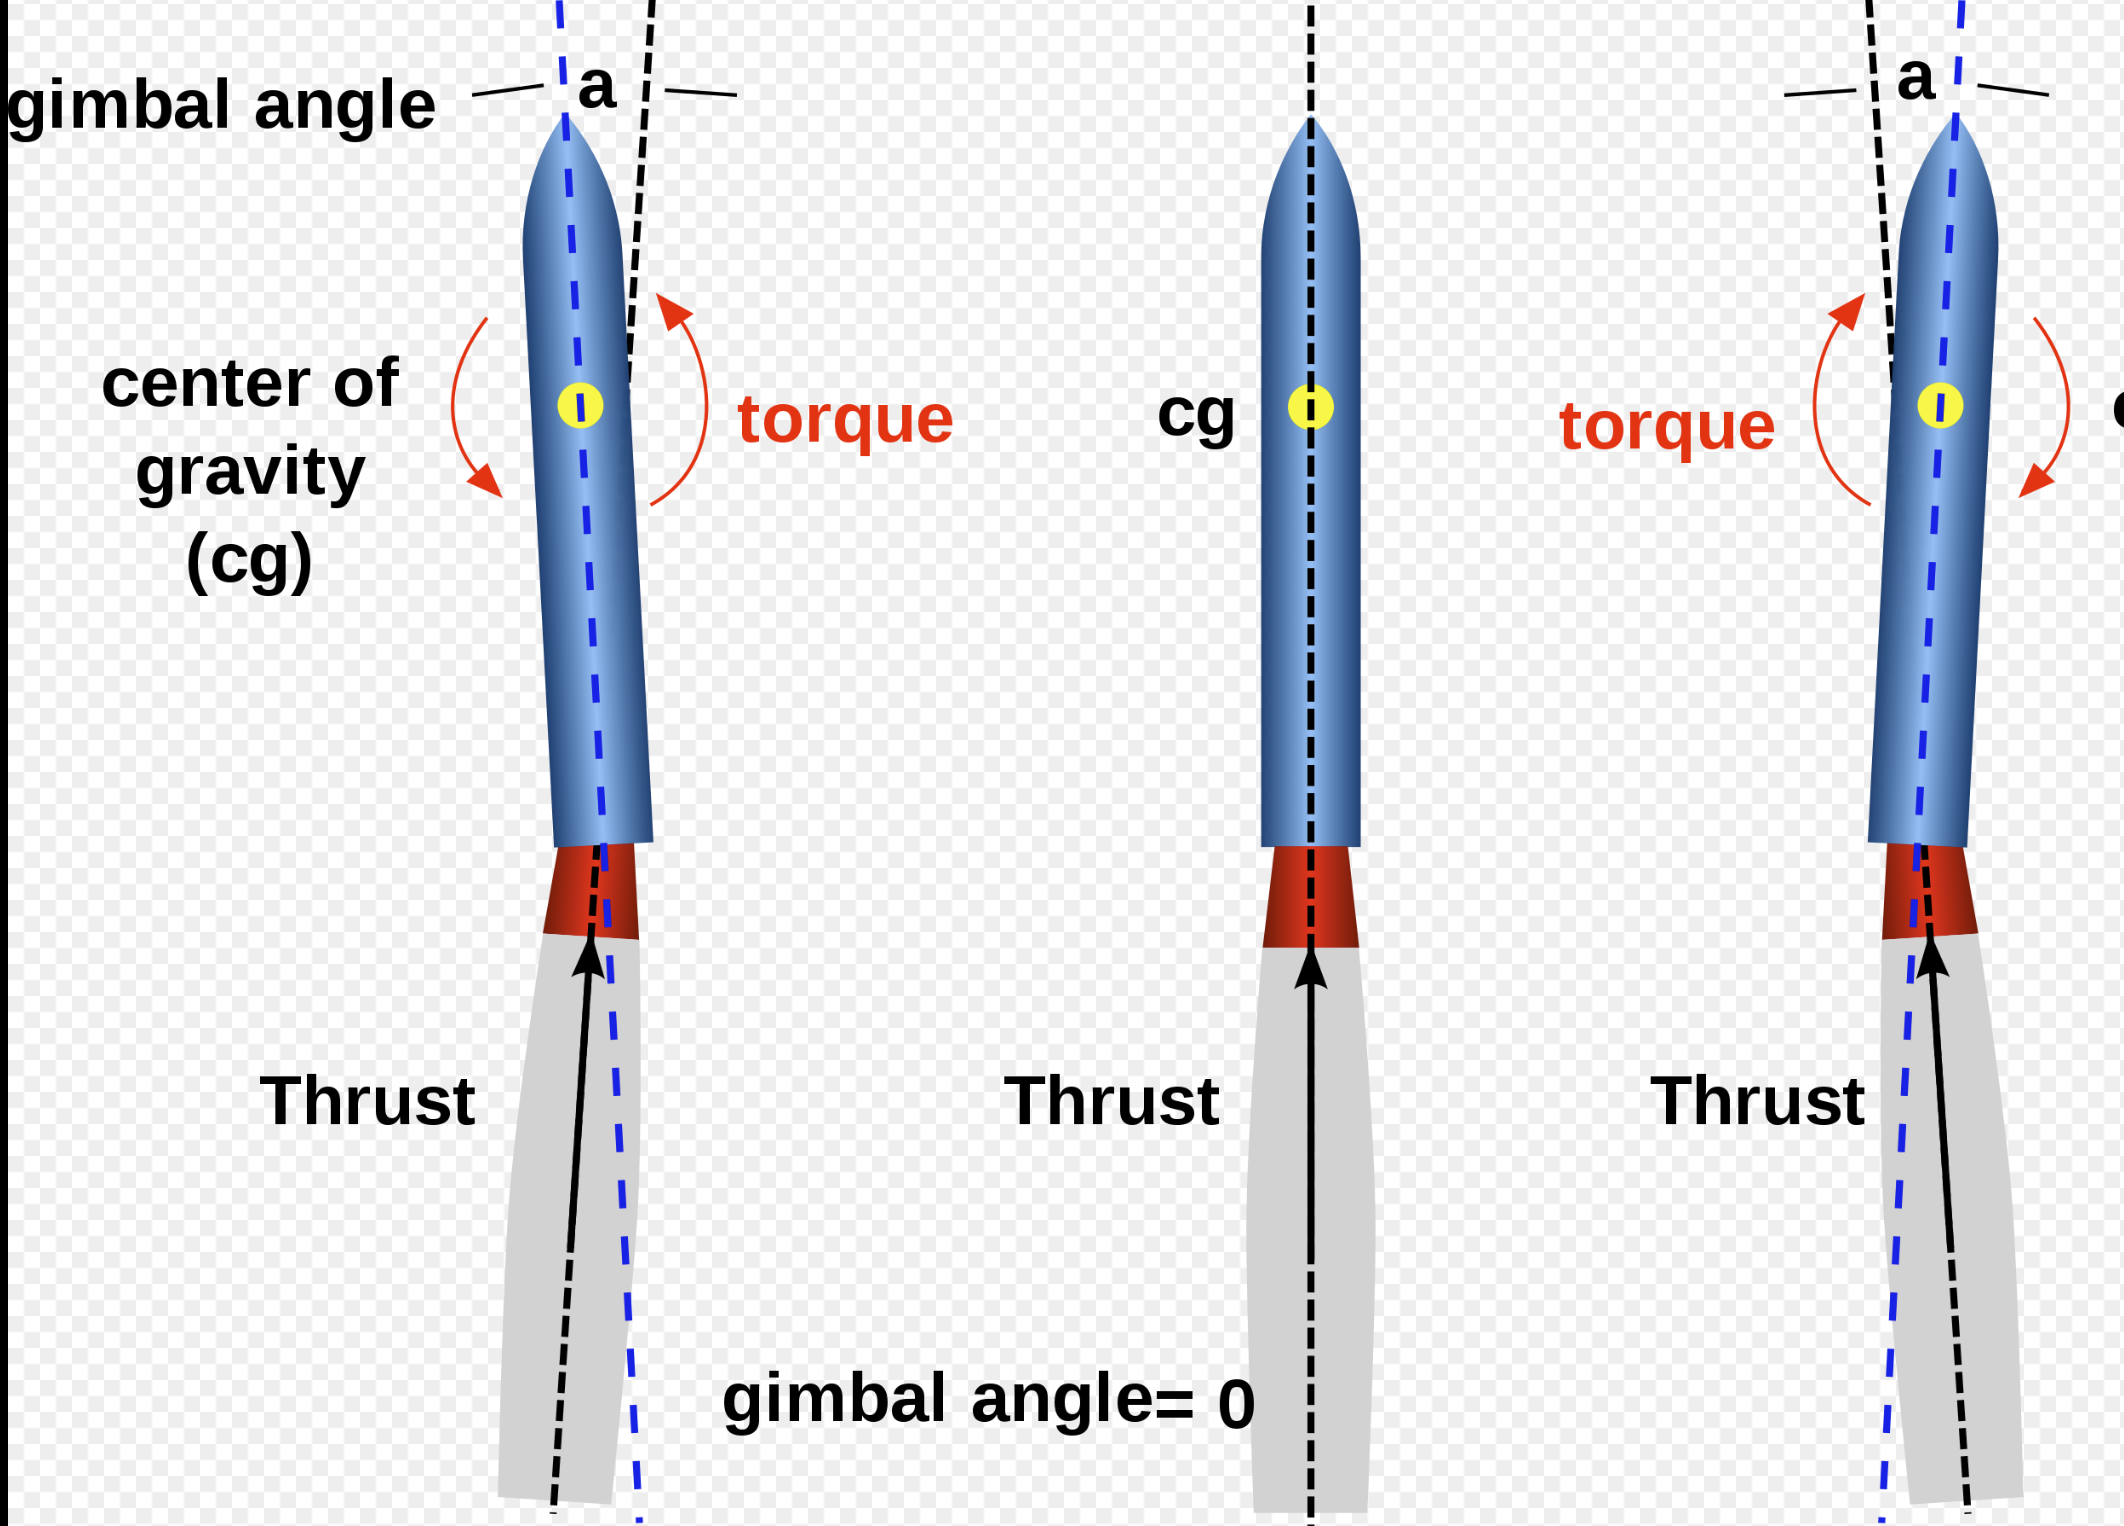
\includegraphics[width=0.5\textwidth]{thrust.png}

\section{Images in Python}
One of the wonderful things about python is the availability of libraries for specialized computation. The Python Imaging Library, PIL, is what you'll use to create images, read existing images from disk, and perform operation on images. To create and manipulate arrays, you will use NumPy. 

Create a file called \filename{image\_creation.py} and enter this code:

\begin{Verbatim}
# Import necessary modules
import numpy as np
import PIL
from PIL import Image
from PIL import ImageOps

# Create a 10 by 10 pixel bitmap Image. 
# Using a decimal point ensure python see the values as floating point numbers
# Some image operations assume floats

bitmapArray = np.array([
[0., 0., 0., 0., 1., 0., 0., 0., 1., 0.],
[0., 0., 0., 0., 1., 1., 1., 1., 1., 1.],
[0., 0., 0., 0., 1., 0., 0., 0., 1., 0.],
[0., 0., 0., 0., 1., 0., 0., 0., 1., 0.],
[0., 0., 0., 0., 1., 0., 0., 0., 1., 0.],
[0., 0., 0., 0., 1., 0., 0., 0., 1., 0.],
[0., 0., 0., 0., 1., 0., 0., 0., 1., 0.],
[0., 0., 0., 0., 1., 1., 1., 1., 1., 1.],
[0., 0., 0., 0., 1., 0., 0., 0., 1., 0.],
[0., 0., 0., 0., 1., 0., 0., 0., 1., 0.]])

# Image.fromarray assumes a range of 0 to 255, so scale by 255

myImage = Image.fromarray(bitmapArray*255)
myImage.show()

# A window opens with an image so tiny you might think nothing is there
# Zoom in to see the pattern  

# Transpose the array, create an image, and then show it. 
# Note that you operate on the original array (not the image)
# Remember to zoom in to see the pattern 

myImageTransposed = bitmapArray.transpose()
myImageTransposed.show()

# Invert the array. You'll use the NumPy invert method.
# The invert method assumes integer values. You need to convert the data type
# Numpy has a method for that

intBitmapArray = np.asarray(bitmapArray,dtype="int")
invertedArray = np.invert(intBitmapArray)

# Take a look at the array

invertedArray

# The values range from -2 to -1. Image values are positive.
# You need to change the range so the values are from 0 to 255
# Further you need to change back to floating point values because
# the PIL method requires them

invertedArray = (invertedArray + 2)*1.0
invertedImage = Image.fromarray(255*invertedArray)
invertedImage.show()

# Zoom in on the image and compare the pattern with the original

\end{Verbatim}

\section{Exercise}

Create a python program that creates matrix $f$ and matrix $g$ from the previous section, and then performs all the operations shown in that section. If you are not sure how to accomplish something, consult the online documentation for the PIL and NumPy python libraries. 
